\documentclass{ctexart}

\usepackage{graphicx}
\usepackage[defaultmono,scale=0.85]{droidsansmono}
\usepackage{amsmath}
\usepackage{amssymb}
\usepackage[hmargin=1.1in,vmargin=1in]{geometry}

\newcommand{\theauthor}{Sparky\_14145}

\input{personal_info/info.tex}

\title{计算机图形 作业五}
\author{\theauthor}

\begin{document}
    \maketitle

    \section{函数流程}

    \subsection{\texttt{Renderer::Render}}

    按照给定参数,计算每一个像素的位置,将从相机所在位置向每一个像素发出的``视线''以后发出并计算最终该像素的颜色,然后将每个像素的结果保存至文件即可。

    需要注意的是枚举像素时,\texttt{i} 对应的是 $x$ 从 0 到画面最大宽度,\texttt{j} 对应的是 $y$ 从 0 到画面最大高度,而相机向 -z 方向看去看到的应该是画面正中央,所以需要把 \texttt{i, j} 缩放到 $[-1, 1]$ 中去,然后再按照说明进行缩放变换。

    另外由于写入文件时像素的写入顺序是由上至下、由左至右,因此在计算坐标时需要将 $y$ 乘上 -1,否则最后渲染结果会上下颠倒。

    \subsection{\texttt{rayTriangleIntersect}}

    直接按照 PPT 上给出的推导结果编写代码进行判定即可。注意如果光线方向与三角面片共面,可以用混合积进行特殊判断处理。

    如果确定有交点,则更新 \texttt{tnear} 为交点对应射线的参数 $t$,\texttt{u}、\texttt{v} 分别为交点的重心坐标。

    \section{运行结果}

    \begin{center}
        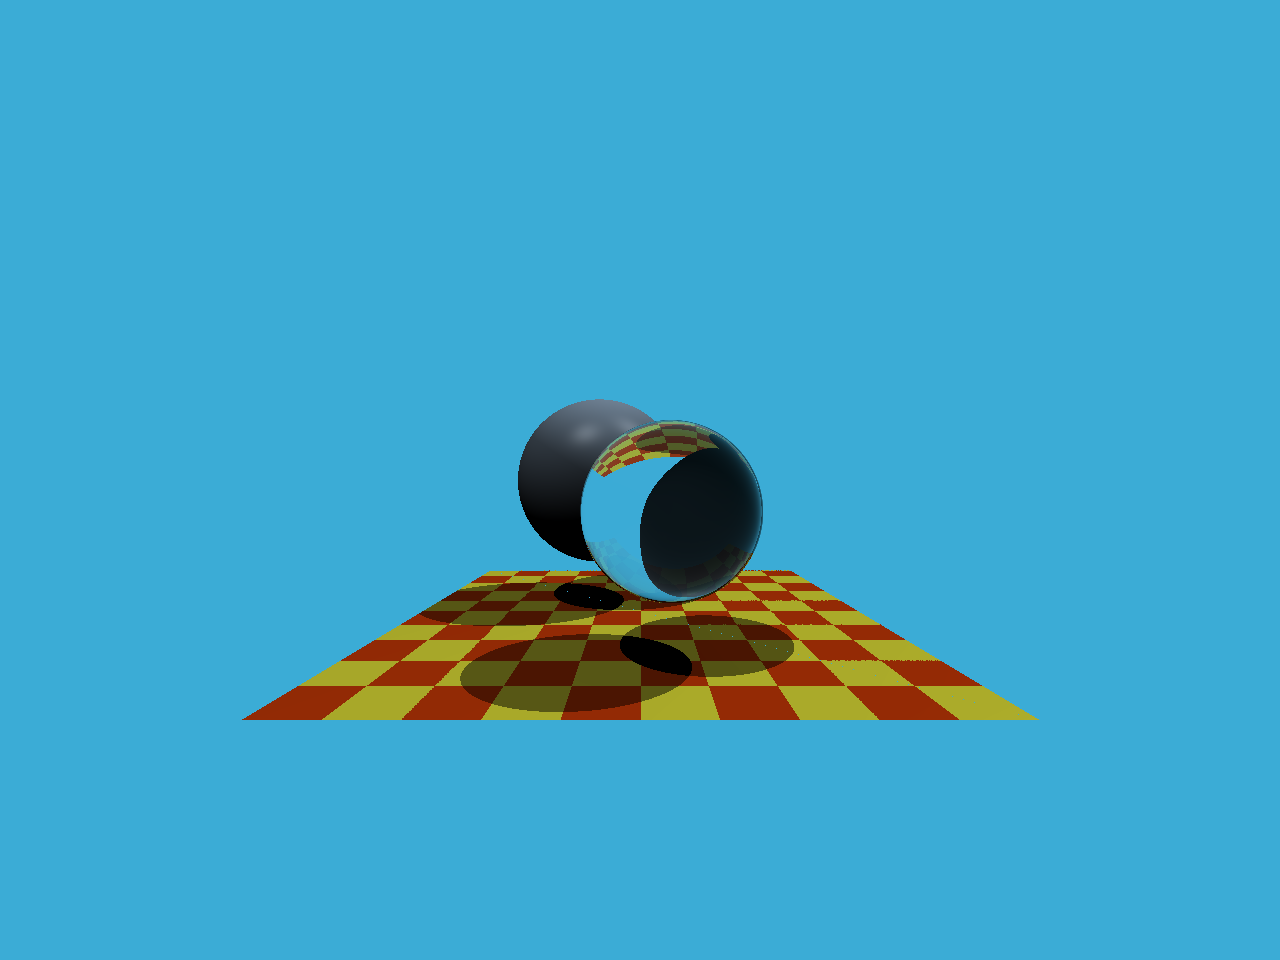
\includegraphics[width=0.5\textwidth]{img/res.png}
    \end{center}
\end{document}